\section{Methoden}

\subsection{Teststrategie}

Wie im Vorsemester im Modul \textit{Software Testing} eingeübt, sollen die \textit{Agile Test Quadrants} (\imgref{fig:agile-testing-quadrants}) als Grundlage zur Erarbeitung einer Teststrategie dienen \cite[p. 242]{agiletest}.

\begin{figure}
	\centering
	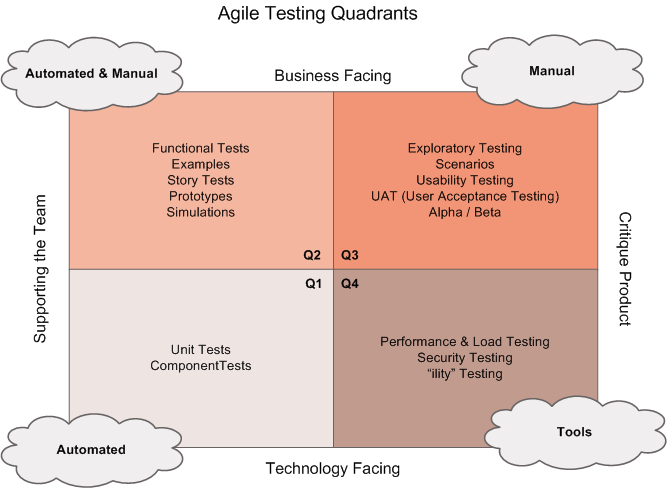
\includegraphics[width=\linewidth]{pics/agile-testing-quadrants.png}
	\caption{\textit{Agile Testing Quadrants} nach Lisa Crispin (\url{https://lisacrispin.com/2011/11/08/using-the-agile-testing-quadrants/})}
	\label{fig:agile-testing-quadrants}
\end{figure}

Für die einzelnen Quadranten bieten sich für das vorliegende Projekte folgende Arten von Tests an:

\subsubsection{Q1: automatisiert}

Im ersten Quadranten geht es um Tests, die vollautomatisch ausgeführt werden können. Diese Tests sollen in einer CI-Umgebung nach jedem Push und vor jedem Merge durchlaufen. Scheitert ein Test, wird der Entwickler notifiziert. Ein Merge-Request soll nicht ausgeführt werden können, wenn Testfälle im Feature-Branch scheitern, sodass die Tests im Master-Branch immer durchlaufen.

Einzelne Funktionen können durch \textit{Unit Tests} abgedeckt werden. Da die Sichtbarkeitsregeln in Go anders geregelt sind als in Java, und ein Unit Test jeweils zum gleichen Modul wie der zu testende Code gehört, können auch interne Funktionen getestet werden, und nicht nur die vom Modul exportierte Schnittstelle \cite[p. 311]{gopl}. Dies erlaubt ein feingranulareres Testing auf Stufe Unit Test.

Die Komponententests sind dann als Tests einzelner Module und somit als Black-Box-Tests zu verstehen, wobei die exportierte (d.h. öffentliche) Schnittstelle angesprochen wird. Auf Mocking soll hierbei verzichtet werden, da das Schreiben \textit{Test Doubles} (Mocks, Spies, Fakes) Kenntnisse der Implementierung und nicht nur der Schnittstelle erfordert. Ändert sich die Implementierung bei gleichbleibendem (und weiterhin erfülltem) Schnittstellenvertrag, sollte auch ein Komponententest weiterhin funktionieren. Dies ist beim Einsatz von Mocks oft nicht gegeben. Eric Elliot bezeichnet Mocking gar als ein \textit{Code Smell}, das die Struktur des Codes verkompliziere, wo doch \textit{Test Driven Development} dabei helfen solle, Code zu vereinfachen \cite[p. 205]{composingsoftware}, 

Ziel der Unit- und Komponententests ist nicht eine möglichst hohe Codeabdeckung, sondern ein optimales Verhältnis von Aufwand und Ertrag: Zeigt es sich, dass für einzelne Tests mit viel Aufwand eine umfassende Umgebung (im weitesten Sinne) aufgebaut werden muss, soll stattdessen geprüft werden, ob der Code nicht besser mittels Tests des zweiten Quadranten getestet werden soll.

\subsubsection{Q2: automatisiert und manuell}

Im zweiten Quadranten geht es um Tests auf der funktionalen Ebene, die teils automatisch, teils manuell ausgeführt werden.

Da \texttt{px} nicht nur interaktiv, sondern auch in Skripten verwendet werden soll, können komplette Workflows ebenfalls vollautomatisiert durchgetestet werden. Ein folgendes Skript könnte etwa folgenden Ablauf beschreiben:

\begin{itemize}
	\item Einloggen auf einen System mit speziellen Test-Zugangsdaten
	\item Hochladen mehrerer Dokumente inklusive Metadaten mit Abspeicherung der dabei generierten Dokument-UUIDs
	\item Tagging der hochgeladenen Dokumente
	\item Herunterladen der zuvor hochgeladenen Dokumente und Vergleich mit dem ursprünglich hochgeladenen Dokument (etwa per SHA-2-Prüfsumme)
	\item Abfragen der zuvor mitgeschickten Metadaten und Tags; Prüfung derselben gegenüber den Ausgangsdaten
\end{itemize}

Ein solcher Test muss zwangsläufig gegen eine laufendes Umgebung durchgeführt werden. (Ähnliche, aber wesentlich einfachere Abläufe werden bereits mit Uptrends durchgeführt, um die Verfügbarkeit der produktiven Umgebung automatisch zu überprüfen.) Hierbei besteht die Gefahr, dass Testfälle aufgrund eines Fehlers in der entsprechenden Umgebung scheitern, und nicht aufgrund der am Code von \texttt{px} vorgenommenen Änderungen. Im schlimmsten Fall müsste ein Merge-Vorgang auf den Master-Branch aufgrund einer nicht funktionierender Umgebung verzögert werden. Eine pragmatische Lösung wäre es, wenn diese Tests gegen die produktive Umgebung ausgeführt würden. Diese Umgebung ist hoch verfügbar, und bei den seltenen Ausfällen derselben könnte auch notfalls mit einem Merge-Vorgang auf den Master-Branch zugewartet werden.\footnote{Der Autor dieser Zeilen ist u.a. auch für die Verfügbarkeit des Produktivsystems zuständig. Ist diese nicht gegeben, werden Entwicklungsarbeiten erfahrungsgemäss unterbrochen, bis das System wieder vollumfänglich verfügbar ist.} Die Zugangsdaten für ein entsprechendes Testkonto können innerhalb der CI-Umgebung als verschlüsselte Variablen und lokal als Umgebungsvariablen abgelegt werden.

Das Schreiben von Skripts ist meistens ein Prozess, dem üblicherweise mehrere manuelle Durchgänge der auszuführenden Arbeitsschritte vorangeht. Skripts werden häufig dann geschrieben, wenn ein manueller Vorgang die Finger stärker beansprucht als den Kopf, und aufgrund der nachgebenden Achtsamkeit die Gefahr für Flüchtigkeitsfehler besteht. So soll es auch im vorliegenden Projekt gehandhabt werden: Wird ein neues Feature eingebaut, d.h. eine neue \textit{User Story} umgesetzt, und sich das Testing desselben als aufwändig herausstellt, soll ein Testskript geschrieben werden, das dann sogleich in die CI-Pipeline eingebaut werden kann. Manuelle Tests sollen so möglichst bald und unkompliziert in automatisierte überführt werden.

\subsubsection{Q3: manuell}

TODO: Usability und User Acceptance Testing (durch Mitarbeiter)

\subsubsection{Q4: Tools}

TODO: Benchmarks, Linter
